\subsection{The Selection of Cities}

Our dataset contains cohorts of individuals raised in Parma and Padova, in addition to Reggio Emilia. Parma and Padova are similar to Reggio Emilia in terms of geography, population, and socio-economic structure, but they do not have the Reggio Approach available.\footnote{Other Italian cities were taken into consideration, notably Brescia, Livorno, Modena, Perugia, Piacenza, Prato, and Ravenna. Parma and Padova were the two cities that best fulfilled our comparability and sample requirements.} 

All three cities are in Northern Italy with Parma and Reggio Emilia being in the same state and Padova being in the neighboring one. In addition to geographic proximity, they have similar populations as seen in Figure~\ref{fig:population}. Although the population in Padova is higher than in Parma and Reggio Emilia, the trends are similar across time. These similar trends can also be seen in the migration rates between the three cities (Figure~\ref{fig:emigr-immigr}). Although emigration rate is highest in Padova and net migration rate is highest in Reggio for most of the years, general trends in emigration and immigration in similar in all cities. Trends in foreign migration are almost identical in three cities. 

The similarities between the cities are also seen in economic terms. Reggio Emilia has an average per-capita income of 25,226 euros, Parma of 28,437, and Padova of 29,915 in 2011 \citep{Comuni-Italiani_2017_Redditi-Ipref-per-Regione-2011}. Other economic information, such as unemployment, is similar across the cities as well. We present more information on the three cities in Appendix~\ref{sec:data-app}.

\begin{figure}[H]
      \centering
        \begin{subfigure}[t]{0.49\textwidth}
          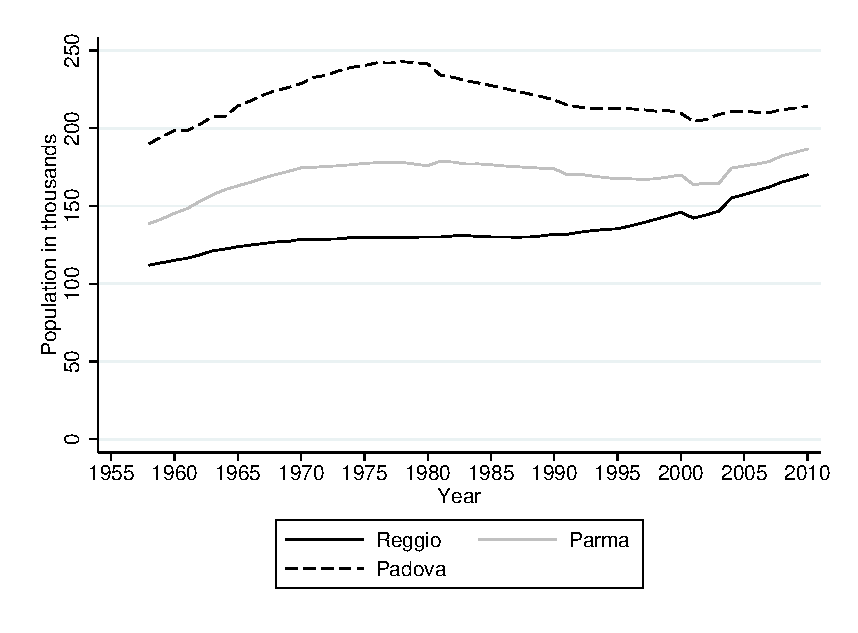
\includegraphics[width=\textwidth]{../../output/image/population.eps}
\caption{Population}
        \end{subfigure}
        \begin{subfigure}[t]{0.49\textwidth}
          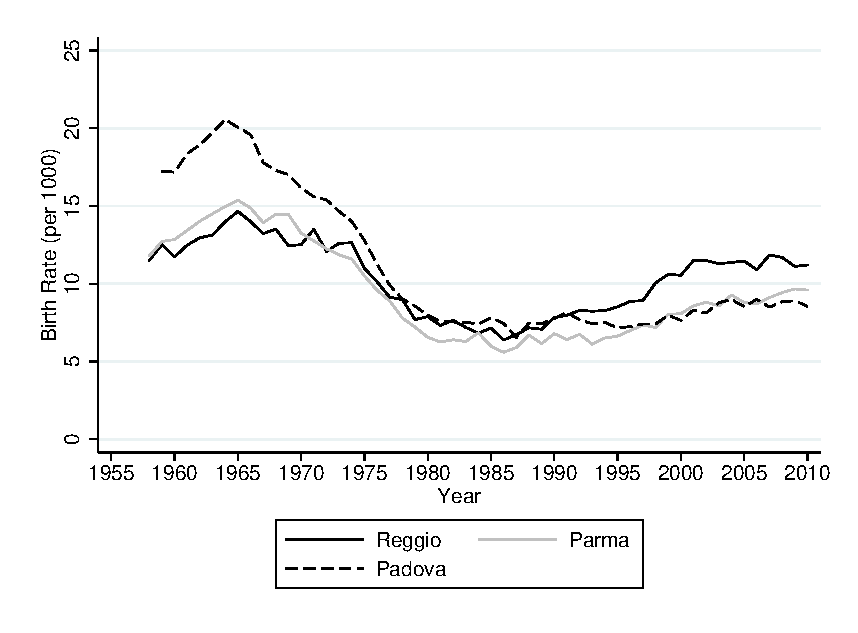
\includegraphics[width=\textwidth]{../../output/image/birth_rate.eps}
 \caption{Birth Rate}
        \end{subfigure}
        \begin{subfigure}[t]{0.49\textwidth}
          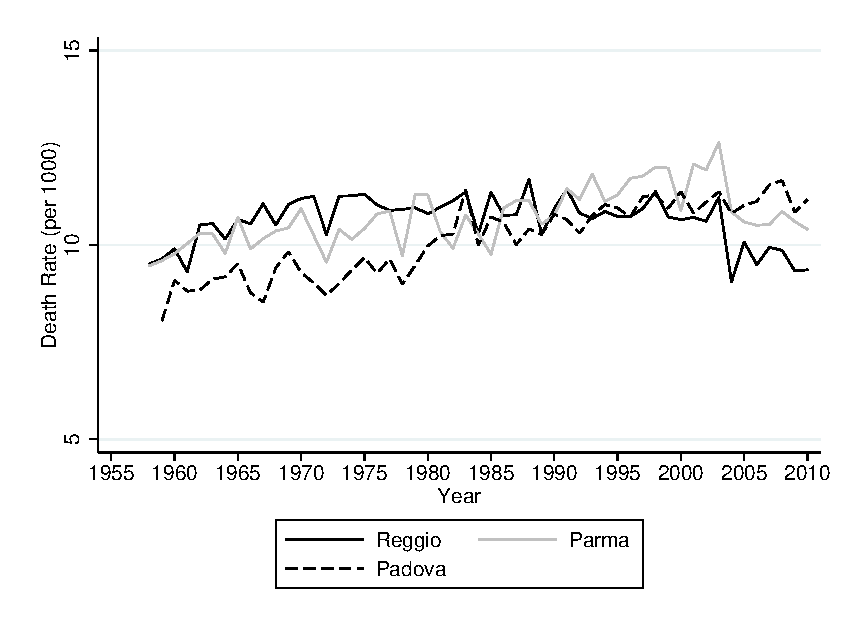
\includegraphics[width=\textwidth]{../../output/image/death_rate.eps}
        \caption{Death Rate}
        \end{subfigure}
        \begin{subfigure}[t]{0.49\textwidth}
          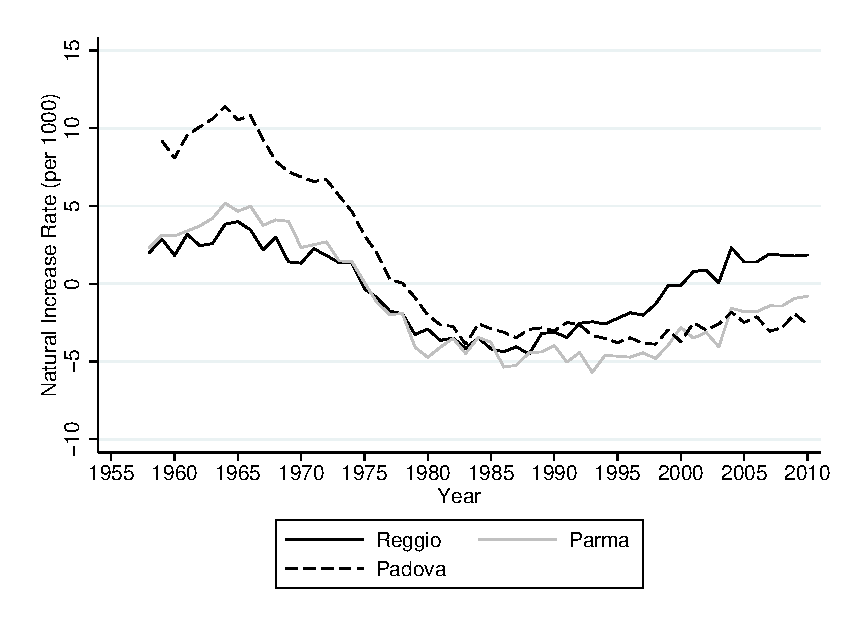
\includegraphics[width=\textwidth]{../../output/image/naturalinc_rate.eps}
            \caption{Natural Rate}
        \end{subfigure}
      \caption{Population Statistics}  \label{fig:population}
    \end{figure}

\textbf{[JJH: Can we test for equality across cities?]}

\begin{figure}[H]
      \centering
        \begin{subfigure}[t]{0.49\textwidth}
          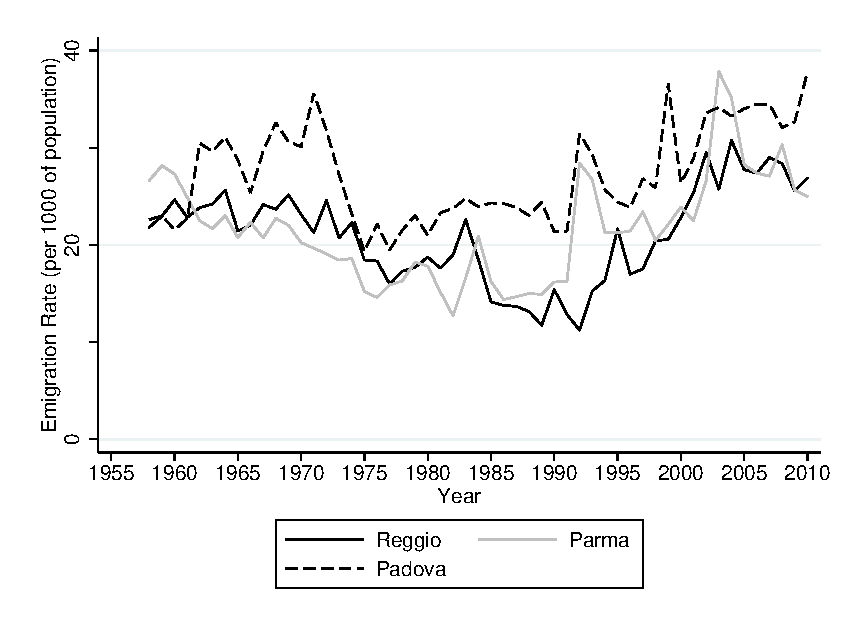
\includegraphics[width=\textwidth]{../../output/image/emigration.eps}
            \caption{Emigration}
        \end{subfigure}
      \begin{subfigure}[t]{0.49\textwidth}
        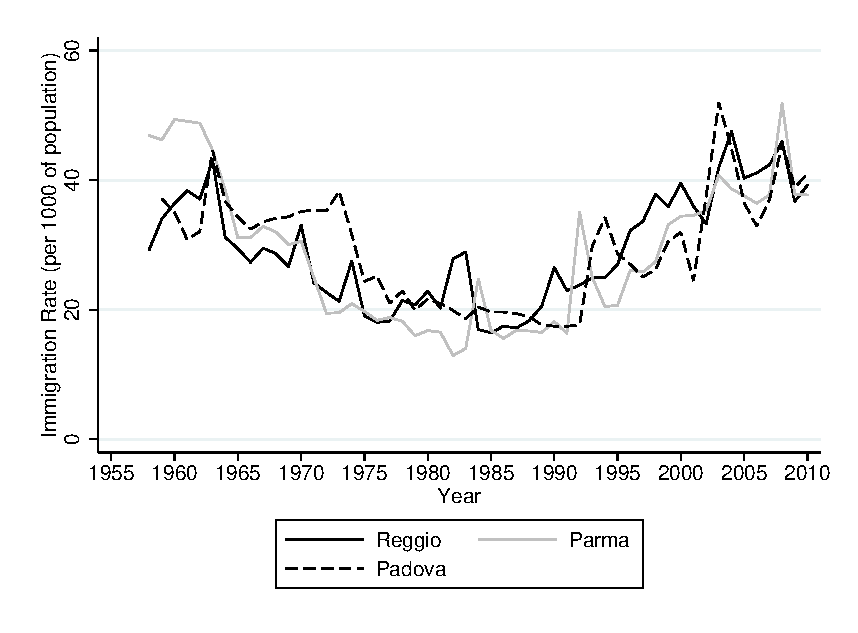
\includegraphics[width=\textwidth]{../../output/image/immigration.eps}
        \caption{Immigration}
      \end{subfigure}
	 \begin{subfigure}[t]{0.49\textwidth}
          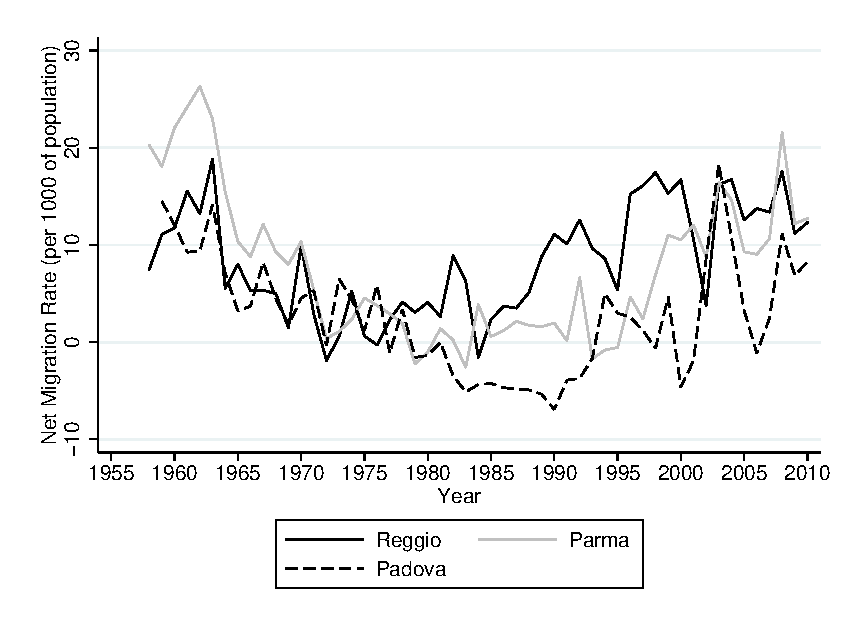
\includegraphics[width=\textwidth]{../../output/image/netmigration.eps}
\caption{Net Migration}
        \end{subfigure}
        \begin{subfigure}[t]{0.49\textwidth}
          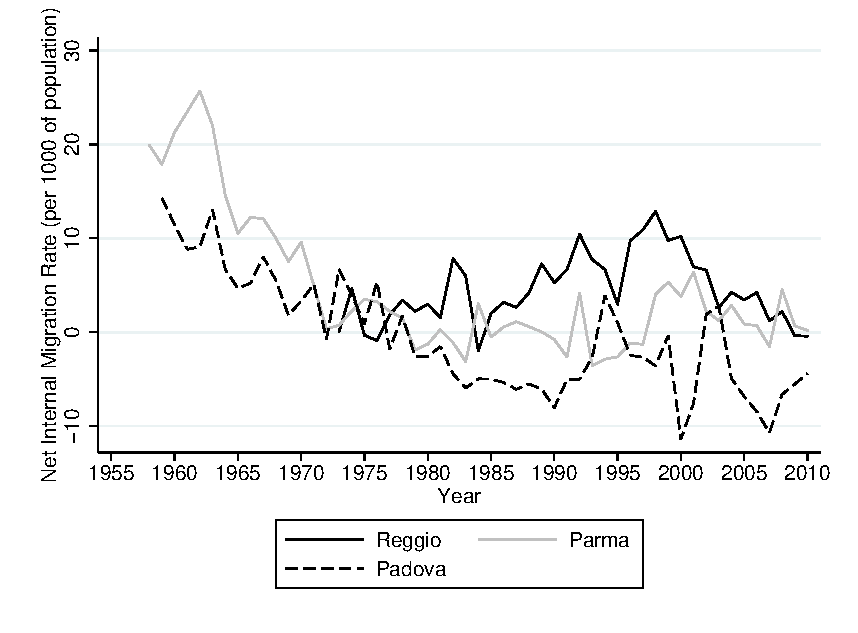
\includegraphics[width=\textwidth]{../../output/image/netinternalmig.eps}
 \caption{Net Internal Migration}
        \end{subfigure}
        \begin{subfigure}[ht]{0.48\textwidth}
          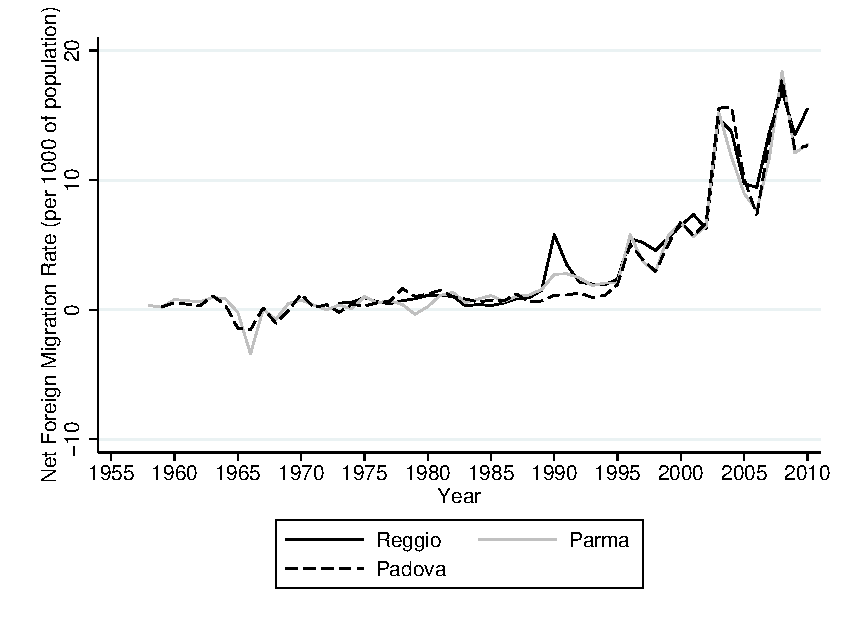
\includegraphics[width=\textwidth]{../../output/image/netforeignmig.eps}
        \caption{Net Foreign Migration}
        \end{subfigure}

      \caption{Migration Statistics}  \label{fig:emigr-immigr}
    \end{figure}